%%%%%%%%%%%%%%%%%%%%%%%%%%%%%%%%%%%%%%%%%
% Stylish Article
% LaTeX Template
% Version 1.0 (31/1/13)
%
% This template has been downloaded from:
% http://www.LaTeXTemplates.com
%
% Original author:
% Mathias Legrand (legrand.mathias@gmail.com)
%
% Modified by:
% Camilo Silva (kamilosilva@gmail.com)
%
% License:
% CC BY-NC-SA 3.0 (http://creativecommons.org/licenses/by-nc-sa/3.0/)
%
%%%%%%%%%%%%%%%%%%%%%%%%%%%%%%%%%%%%%%%%%

%----------------------------------------------------------------------------------------
%	PACKAGES AND OTHER DOCUMENT CONFIGURATIONS
%----------------------------------------------------------------------------------------

\documentclass[fleqn,12pt]{NTFD} % Document font size and equations flushed left

\setlength{\columnsep}{0.55cm} % Distance between the two columns of text
\setlength{\fboxrule}{0.75pt} % Width of the border around the abstract

\definecolor{color1}{RGB}{0,0,90} % Color of the article title and sections
\definecolor{color2}{RGB}{0,20,20} % Color of the boxes behind the abstract and headings

\newlength{\tocsep} 
\setlength\tocsep{1.5pc} % Sets the indentation of the sections in the table of contents
\setcounter{tocdepth}{3} % Show only three levels in the table of contents section: sections, subsections and subsubsections



\usepackage{lipsum} % Required to insert dummy text
\usepackage{setspace} % To add space between lines
\onehalfspacing
\linespread{1.1}

\usepackage{fourier}
\usepackage{physics}
\usepackage[T1]{fontenc}
\usepackage{subcaption} % for pictures side by side
\usepackage{listings} % for code blocks
\usepackage{float} % force figure positions



%----------------------------------------------------------------------------------------
%	ARTICLE INFORMATION
%----------------------------------------------------------------------------------------

\Archive{Winter Semester 2020-2021} % Period of course

\PaperTitle{2D wave propagation in different irregular geometries} % Article title

\Authors{Sebastian Egger\textsuperscript{1}*, Adrian Salah\textsuperscript{2}} % Authors
\affiliation{\textsuperscript{1}\textit{Master Student, TUM, Munich, Germany}} % Author affiliation
\affiliation{\textsuperscript{2}\textit{Master Student, TUM, Munich, Germany}} % Author affiliation
\affiliation{*\textbf{e-mails}: sebastian.egger@tum.de,\  adrian.salah@tum.de} % Corresponding author

\Keywords{wave equation --- finite volume method --- wave propagation} % Keywords - if you don't want any simply remove all the text between the curly brackets
\newcommand{\keywordname}{Keywords} % Defines the keywords heading name

%----------------------------------------------------------------------------------------
%	ABSTRACT
%----------------------------------------------------------------------------------------

%\Abstract{\lipsum[1]~}
\Abstract{ In this work the authors investigated the transmission of waves through different geometries using the wave equation. The geometries of interest are three variations of the popular `Backstep' geometry that is often used in computational fluid dynamics to visualize turbulence phenomenon. The variations differ in the transition of the inlet to the outlet. Goal of this work is to find out how the difference in the transition affects the wave propagation. The input signal is a random noise signal generated at the inlet. The observation of the experiments showed that a sharp corner results in more waves being reflected while a smooth transition allows for a better wave transmission. The authors also used a spectral analysis of the wave amplitudes at specific probe positions in the domain to get insight over the resonance behaviour of the geometry.
}


%----------------------------------------------------------------------------------------

\begin{document}

\begin{titlepage}

\begin{figure}

\includegraphics[width=2cm]{./Logo.pdf}
\end{figure}

\end{titlepage}


\flushbottom % Makes all text pages the same height

\maketitle % Print the title and abstract box

\newpage

\tableofcontents % Print the contents section

\thispagestyle{empty} % Removes page numbering from the first page

%----------------------------------------------------------------------------------------
%	ARTICLE CONTENTS
%----------------------------------------------------------------------------------------

\section{Introduction} % The \section*{} command stops section numbering

%\addcontentsline{toc}{section}{\hspace*{-\tocsep}Introduction} % Adds this section to the table of contents with negative horizontal space equal to the indent for the numbered sections

% 1) Description of the problem
% musical instruments 
% resonance, harmonics
The studied phenomenon of interest is a wave propagating through different cone shaped geometries displayed in figure \ref{fig:geometries}.

\begin{figure}[ht]\centering % Using \begin{figure*} makes the figure take up the entire width of the page
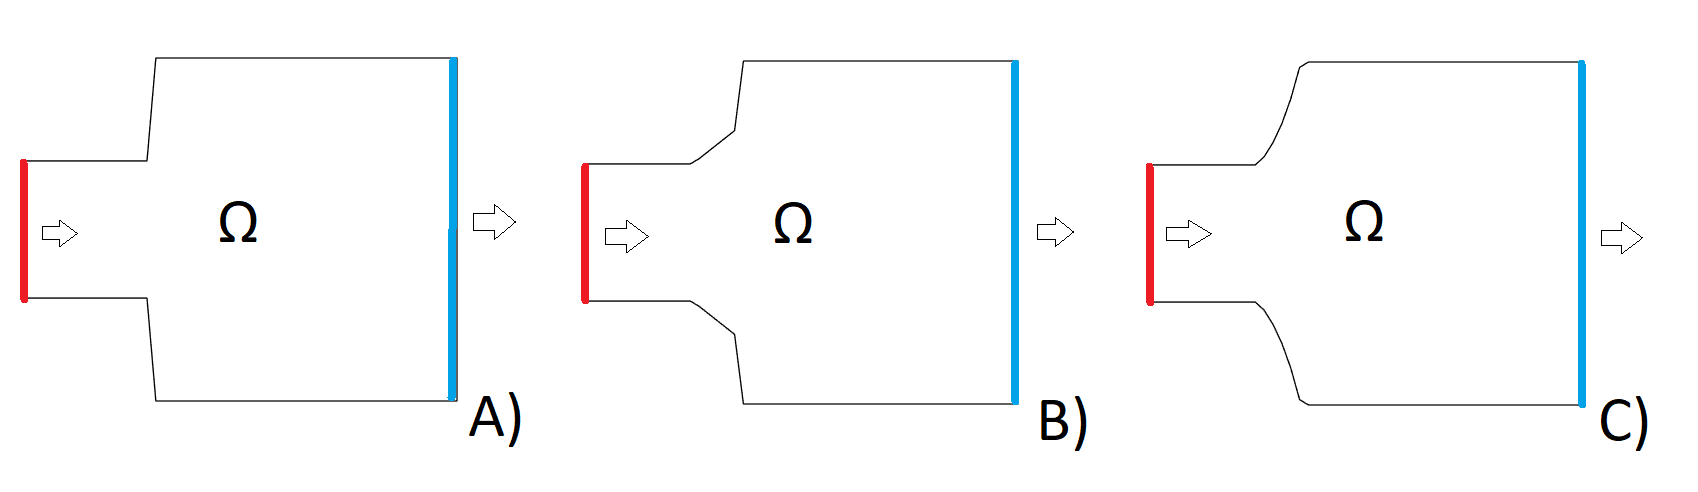
\includegraphics[width=\linewidth]{geometries.png}
\caption{Outline of the studied geometries. The inlet is marked in red and the outlet in blue colour. The geometries are referred to as A) Backstep, B) angled Backstep and C) smooth Outlet }
\label{fig:geometries}
\end{figure}

A white noise signal is fed into the inlet. It shall be investigated which frequency fractions are propagated through the inlet tube into the higher volume outlet chamber and which ones are reflected . Moreover it is examined if resonance is emerging and how those phenomena depend on the chosen geometry setup. 

As a real world example one could imagine a wind instrument. Pressure differences created at the mouthpiece induce a longitudinal wave propagating through the instrument. The geometry of the instrument influences the created sound and therefore determines the frequencies leaving the outlet. \\
For this task a FVM solver for the two dimensional wave equation was developed. 
% 2) Physical description (without too much mathematics) of the phenomenon
% intro wave equation
The wave equation is important for various branches of science and engineering such as fluid dynamics, acoustics, electro-magnetics or geophysics to name just a few.
For this problem we consider the homogeneous wave equation. It is a second order partial differential equation (PDE) of the form:
\begin{equation} \label{eq:wave equation}
 \pdv[2]{u(\vb{x},t)}{t} - c^2 \grad ^2 u(\vb{x},t) = 0
\end{equation}

Therefore we have no source (or sink) terms in our simulation domain $\Omega$.
The scalar quantity $u$ %is the propagated physical quantity. 
can generally represent different physical quantities. We consider $u$ to be a  scalar pressure field $p(\vb{x}, t)$.
In equation \ref{eq:wave equation}, $c$ corresponds to the propagation speed or \emph{phase velocity} of the wave. Evidently the phase velocity depends on the medium and its state through which the wave is propagating.
% hyperbolic 
From the general form of a linear second ordner PDE of two independent variables $(x,t)$ \cite{CamiloF.SilvaPh.D..2020}
\begin{equation} \label{eq: lin_pde}
A \pdv[2]{\phi(x,t)}{t} + B \pdv[1]{\phi(x,t)}{t}{x} + C \pdv[2]{\phi(x,t)}{t} + ... =  0
\end{equation}
we can easily see that the expression $B^2 - 4AC$ is always bigger than zero as $B = 0$ and $C = -c^2 <0$ in case of the wave equation. This argument can be extended to higher spatial dimensions $\vb{x} =  (x,y,...)$ as well. Thus, the wave equation is a \emph{hyperbolic} PDE. 
% solution of the wave equation 
%1D than higher dimensions
% our analysis, initial boundary conditions
We want to restrict the analysis to the two-dimensional case. The wave equation consequently takes the from $ p_{tt} - c^2( p_{xx} + p_{yy}) = 0$. 
%Here $p_{**}$ denotes the second partial derivative with respect to the variable $*$. 


%------------------------------------------------

\section{Discretization}
In order to solve this PDE on a computer, the computational domain needs to be discretized. The discretization needs to be in space as well as in time.
\subsection{Spatial discretization}
To discretize the spatial domain, the finite volume method was used. The domain is divided into cells with nodes at the corners. The PDE is integrated over each cell and using greens theorem we can find relations between each cell and neighbouring cells. This results in the discretized operator for the spatial discretization $Au_n=b$, which is a linear system of equations we can solve on the computer. 

We used different geometries to solve the wave equation and compare the results. There are multiple ways of solving the PDE on a given geometry using a structured mesh. The first option is to use one mesh which is non-uniform over the domain. \\
The second option is to use two meshes (two separate domains) and connect them via the boundary conditions (outlet values of one domain are used as inlet values for the second domain) and if necessary the values are interpolated. \\
The third option is to use a rectangular domain as big as necessary to cover the given geometry and then only use the nodes that lie within the geometry for computation. 

In our case we chose the third option for our mesh. In order to realize this approach the dummy nodes (nodes that are not used in the computation) as well as the boundary nodes have to be determined. In our case only the boundary nodes on the north boundary had to be determined as the other boundary nodes are just at the boundary of the rectangular domain. 

\begin{figure}
    \centering
    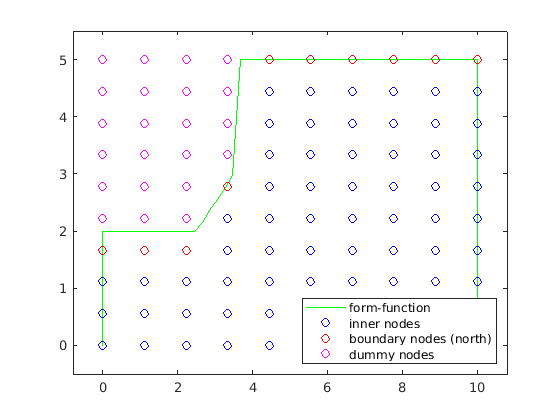
\includegraphics[width=0.7\textwidth]{mesh.png}
    \caption{This figure shows the form-function of the given geometry and the nodes of the mesh}
    \label{fig:mesh}
\end{figure}

Figure \ref{fig:mesh} shows our mesh and the different nodes in different colours. The domain is a rectangular domain with a Cartesian mesh. The green line indicates the form-function which shows the given geometry. The purple nodes show the dummy nodes, which are not used in the computation. The red nodes are the nodes that are assigned to the north boundary and the blue nodes are the inner nodes (and also nodes belonging to other boundaries than the north boundary). 

The advantage of our approach is that we can avoid stability issues that are introduced with cells that have different sizes as all of our cells have the same size but we do not use all of the cells for the computation.
\subsection{Time discretization}
The wave equation is an unsteady problem which means we have an evolution in time. For the computation we use a temporal domain $t \in [0, t_{end}]$ with equidistant time-step sizes $\Delta t = t_1 - t_0 = t_n - t_{n-1}$.
The discretization of the PDE in time is handled via finite differences. For the wave equation we have a second-order time derivative, which allows the use of the centered difference approximation:

\begin{equation}
\frac{\partial^2}{\partial t^2} u \approx \frac{u_{n-1} - 2u_n + u_{n+1}}{\Delta t^2}
\end{equation}
The centered difference scheme is second order accurate in time so $\mathcal{O}(\Delta t^2)$.
The update rule to compute the solution of the wave equation for each time step can be written as follows,
\begin{equation}
u_{n+1} \approx 2u_n - u_{n-1} + c^2 \Delta t^2 (Au_n -b)
\end{equation}
with $Au_n-b$ being the discretized version of the Laplacian operator.

One might recognize that for the solution of the next time step, the solution of the current as well as the past time-step are needed. Then the question arises how we can compute the first time step with only the current (zeroth) time-step. As this is not possible we find that we need not only an initial condition for the value $u_n$ at time $t = 0$, but also for the derivative $u'_n$ at time $t = 0$. Using the initial condition $u'_n = 0$ and a forward difference scheme for the approximation of the derivative we get the following expression:
\begin{equation}
    \frac{u_0 - u_{-1}}{\Delta t} = 0
\end{equation} 
with the timestep size $\Delta t$.
This results in the following condition $u_0 = u_{-1}$. Using this discretization scheme we only get first order accuracy in time $\mathcal{O}(\Delta t)$. As we mix a second order discretization scheme with a first order discretization scheme we can only expect the solution to be first order accurate in time.


\subsection{Numerical stability}

% check this again!
The numerical stability of this method shall be investigated in the following. As our computational domain $\Omega$ is a rectangle with fixed cell-lengths $\Delta x $ and $\Delta y$ we can derive a stability criterion by means of the von Neumann stability analysis. The general solution of the wave equation \ref{eq:wave equation} can be obtained by adding complex Fourier components 
\begin{equation} \label{fourierdecomp}
  u (\vb{x},t) =\sum_{n=0}^{\infty}  a_{n} e^{i(k_x  \Delta x + k_y \Delta y - \omega \Delta t)}
\end{equation} 
% k is wave vector ...
% omega is angular frequency
We use uniform timesteps: $t = n \Delta t $ for $n = \{0,1,2,3,...\}$ as well as equidistant grid points $x = l \Delta x $ and $y =m \Delta y $ with $m = \{0,1,2,3,...\}$ and $l = \{0,1,2,3,...\}$. \\
Therefore we can express the discretized solution as:

\begin{equation}
  u^n_{l,m} =\sum_{n=0}^{\infty}  a_{n} e^{ik_x l \Delta x} e^{ik_y m \Delta y}e^{ -i \omega n \Delta t}
\end{equation} 

The discretized wave equation can now be written as:

\begin{equation} \label{eq: wave_equation_discretized}
D^2_{t} u^n_{l,m} = c^2 [D^2_{x} + D^2_{y}] u^n_{l,m}
\end{equation} 


The error between the exact solution at the grid points $u(x_l, y_m, t_n)$  and the discretized solution $u^n_{l,m}$ is defined as $\epsilon^n_{l,m} = u^n_{l,m}  - u(x_l, y_m, t_n)$. As $u^n_{l,m}$ and $u(x_l, y_m, t_n)$ satisfy the discretized wave equation exactly, the error also  satisfies equation \ref{eq: wave_equation_discretized}.
For stability it is required that the error amplification factor:

\begin{equation} \label{eq:amplification factor}
 G := \frac{\epsilon^{n+1}_{l,m}}{\epsilon^n_{l,m}} \stackrel{!}{<} 1 
\end{equation}

That essentially means that the error terms do not grow with time.
% why does the error satisfy the equation as well?
% why to I need just a single component
Applying the discrete operators $D^2_{t}, D^2_{x}$ and $D^2_{y}$ on one single component of $u^n_{l,m}$ we obtain after some calculation:

\begin{equation}
sin^2 \Bigg ( \frac{\omega \Delta t}{2}\Bigg) = {\Bigg ( \frac{c \Delta t}{\Delta x} \Bigg)}^2 sin^2 \Bigg( \frac{k_x \Delta x}{2} \Bigg) + \Bigg(\frac{c \Delta t}{\Delta x}\Bigg)^2 sin^2 \Bigg(\frac{k_y \Delta y}{2} \Bigg)
\end{equation}
% explain this !
To full-fill the stability criterion in Eq. \ref{eq:amplification factor} we need to satisfy following relation: 

\begin{equation} \label{eq:stability criterion}
\Delta t < \frac{1}{c} \Bigg(\frac{1}{\Delta x^2} + \frac{1}{\Delta y^2} \Bigg)^{-1/2}
\end{equation}

This condition is checked in the code for the specified parameters after the initialisation in the file \texttt{InitFVM.m}  by the function \texttt{isWaveStable()}. If the condition \ref{eq:stability criterion} evaluates to \texttt{False} an error is thrown. A message that the CFL condition is not met is displayed to the user. This ensures robustness of the provided code. 

In figure \ref{fig:instability} we provide an example of a developing instability of the solution after a certain time-step. Note that the phase velocity $c$ also influences the stability of the algorithm. The analysis was restricted for a constant phase velocity $c = const$. However it can be in general be extended to variable phase velocities $c(\vb{x})$. For non-constant phase velocities the worst-case absolute velocity $\tilde{c}$ value has to be considered.  $$ \tilde{c} = \sqrt{\max_{{\vb{x}} \in \Omega}{( c^2(\vb{x})})}$$
For this case an additional safety factor  $\beta < 1$ is often used. This was not done in the developed code as the phase velocity $c$ is fixed. This loosens additional restrictions on possible parameter choices. The presented stability analysis can be conveniently extended to three dimensions. 


\begin{figure}[ht]\centering % Using \begin{figure*} makes the figure take up the entire width of the page
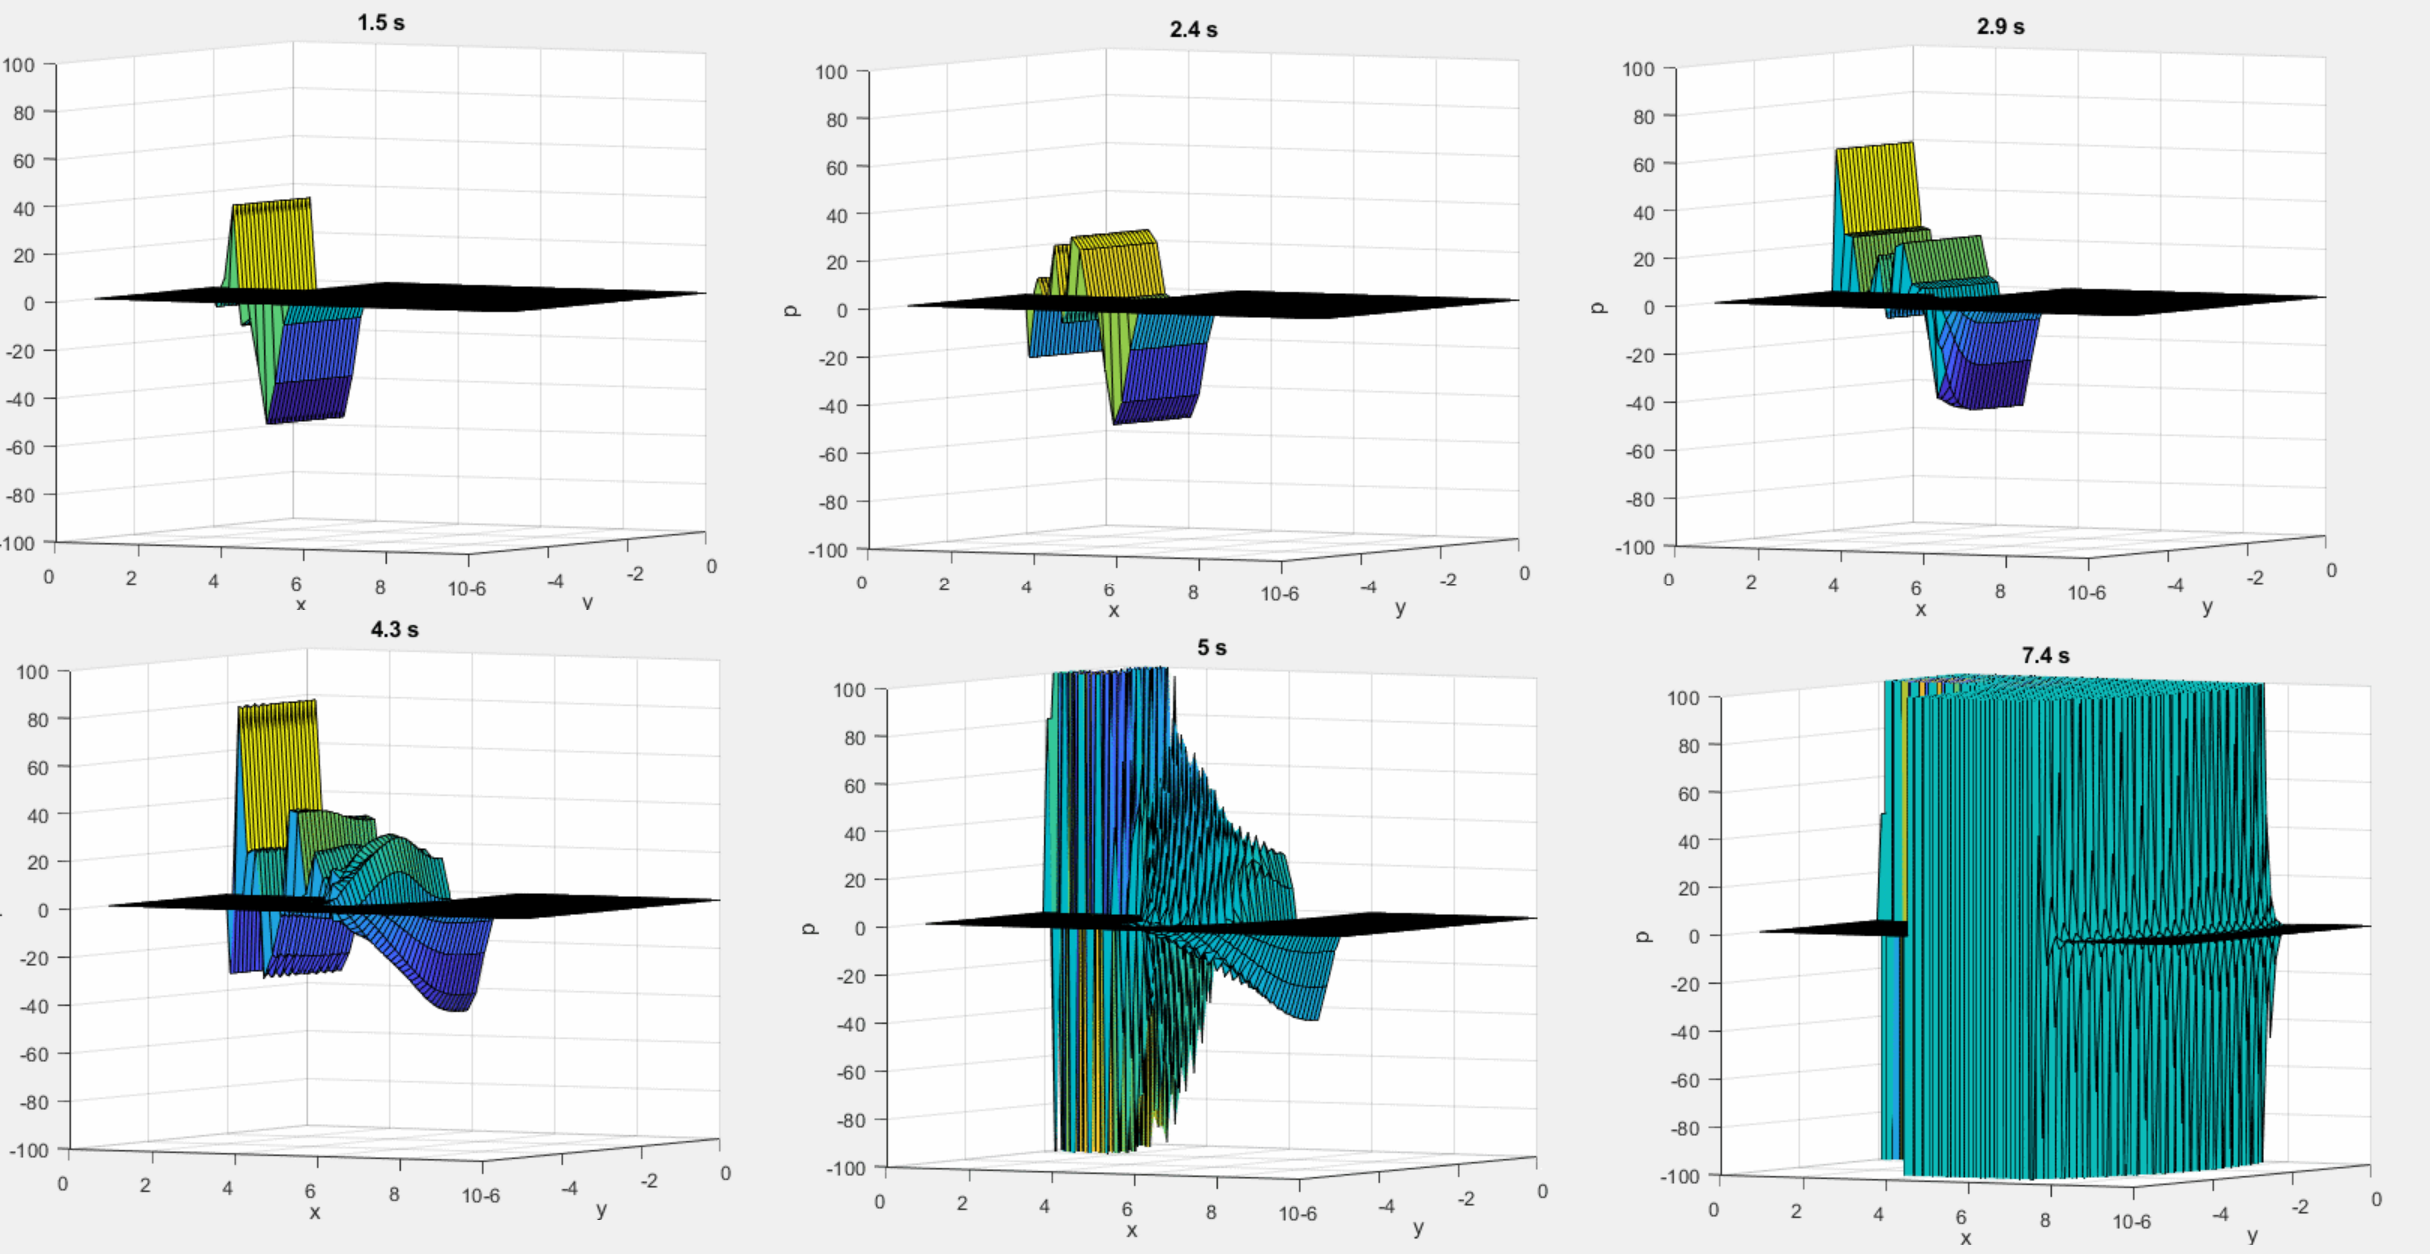
\includegraphics[width=\linewidth]{instability.png}
\caption{Development of a numerical instability for parameter choice $\Delta x = 0.2, \ \Delta y = 0.1, \ c = 1 $ and $dt = 0.1$. The stability criterion in equation \ref{eq:stability criterion} is not fullfilled. Therefore the solvercode would throw an error in this case}
\label{fig:instability}
\end{figure}


\section{Boundary Conditions}
The process of solving a given PDE has to be handled differently at the boundary than at the inner nodes of the computational domain. To specify the solution behaviour at the boundary we use boundary conditions.

There are three different types of boundary conditions, homogeneous Dirichlet, homogenous Neumann and Robin boundary conditions. Dirichlet BCs use a fixed value of the solution e.g. $u = 0$ on the boundary, Neumann BCs use a fixed gradient of the solution e.g. $\frac{\partial}{\partial x}u = 0$ and Robin BCs are a combination of Dirichlet and Neumann BCs.

\subsection{Physical meaning of boundary conditions}

Regarding the wave equation there are different physical phenomenons related to the different types of boundary conditions.
The homogeneous Dirichlet boundary condition applied on a boundary, will result in the wave being reflected off the boundary but with the opposite sign and a fixed amplitude value of zero on the boundary.
The homogeneous Neumann boundary condition applied on a boundary will result in the wave being reflected off the wall with the same sign.
One special Robin boundary condition is the so called open boundary condition. It allows a wave to exit the computational domain without any other interaction. Depending on the direction of the wave the open boundary condition can be formulated as follows:
\begin{equation}
    \frac{\partial u}{\partial t}+c\frac{\partial u}{\partial x}=0
\end{equation}
It can be shown that the above equation accepts a solution $u=g_R(x-ct)$ (right-going wave), but not $u=g_L(x+ct)$ (left-going wave). This means the above equation will only allow right-going waves to pass through the boundary undisturbed.

\subsection{Boundary Conditions used in our case}

With the physical meaning of the boundary conditions explained we can discuss the boundary conditions used in our case setup. We used the west boundary as our inlet and the east boundary as our outlet. Because we exploited symmetry to save computational costs we use the south boundary as our symmetry boundary. The north boundary governs the shape of our geometry.

To simulate an incoming signal at the inlet, we use a time-dependent Dirichlet boundary condition on the west boundary. To make the signal travel through the geometry and out into the open without reflecting into the domain, we used the open boundary condition on the east boundary. For the symmetry on the south boundary we used a homogeneous Neumann boundary condition. We used the same boundary condition for the north boundary but instead of simulating a symmetry boundary we simulate a reflecting wall. Figure \ref{fig:boundary} gives a visual overview over the boundary conditions that are used in our case.
\begin{figure}
    \centering
    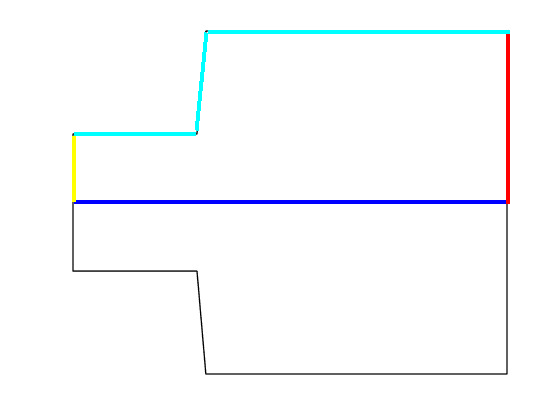
\includegraphics[width=0.5\textwidth]{boundary.png}
    \caption{This figure shows the boundaries of the domain. \textbf{Blue:} Symmetry boundary with homogeneous Neumann BC. \textbf{Yellow:} Inlet boundary with time-dependent Dirichlet BC. \textbf{Red:} Outlet boundary with open-boundary condition. \textbf{Cyan:} North boundary specifying the shape of the geometry with homogeneous Neumann BC}
    \label{fig:boundary}
\end{figure}


\section{Implementation}
In this section the essential components of the implemented code and solver steps are outlined.
In the script file \texttt{InitFVM.m} all relevant physical parameters are defined. This includes mesh dimensions, time-step size, simulation time and choosen geometry among other parameters. It can be also specified how long the time-depended (white noise) input signal is present during the simulation time. 

A setup file is stored to the project directory to store all the relevant parameters of the simulation.
In the function \texttt{setupMesh()} the mesh nodes are initialized. Depending on the chosen geometry based on the form-function nodes outside of the simulation domain $\Omega$ are labeled as `dummy nodes'. 

The main solver loop consists of one loop to set up the coefficient matrix $A$ of the spatial discretization according to the finite volume method as presented above. As $A$ is a static matrix it should be avoided to initialize $A$ at every solution time-step for memory and performance reasons. For this matter the \texttt{stamp()} function, which previously calculated $A$ and right hand side vector $b$ was split up in two separate functions. 

In line 1-8 the coefficient matrix is set up. If the current mesh node is a `dummy node' as defined in the function \texttt{setupMesh()} it results in a zero line in the coefficient matrix $A$. Fig.~\ref{fig:matrix structure} displays the structure of $A$ for a different number of mesh nodes. The highly sparse tridiagonal structure of $A$ suggests storing it in a sparse format.


% time plot, spectrum backstep, inlet 
\begin{figure}
\centering
\begin{subfigure}{.5\textwidth}
  \centering
  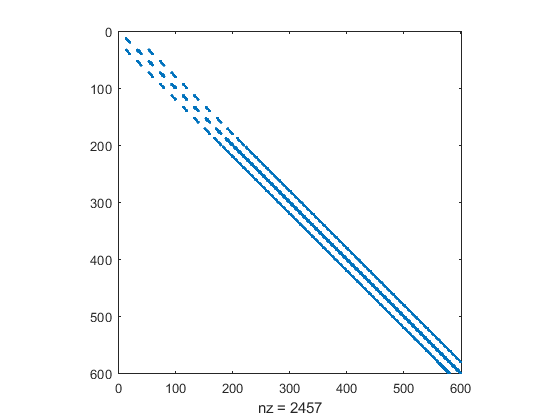
\includegraphics[width=.8\linewidth]{matrixA2030.png}
  \caption{$dimX = 20, \ dimY = 30$}
  \label{fig:A2030}
\end{subfigure}%
\begin{subfigure}{.5\textwidth}
  \centering
  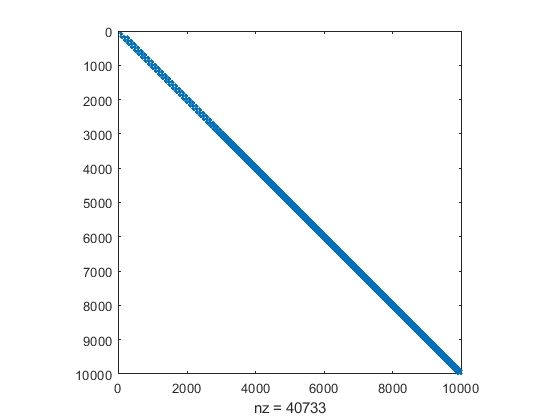
\includegraphics[width=.8\linewidth]{matrixA100100.png}
  \caption{$dimX = 100, \ dimY = 100$}
  \label{fig:sub2}
\end{subfigure}
\caption{Coefficient matrix $A$ for different spatial resolutions}
\label{fig:matrix structure}
\end{figure}

 In the next loop the right hand side vector is calculated according to the defined boundary conditions. If the current mesh node is a `dummy node' as defined in the function \texttt{setupMesh()} it is ignored for the calculation.
For the east side open boundary condition the first time derivative has to be calculated and passed to the \texttt{rhs()} function. The \texttt{rhs()} function is responsible for calculating the right hand side vector of the system $Ax=b$ based on the imposed (and now time depended) boundary conditions. Likewise the current time-step has to be passed to \texttt{rhs()} to take account for the time-depended Diriechlet Boundary condition on the west-side. In the following the main solution step is executed and the current solution is stored in the solution array. Finally the variables and boundaries of the solution are updated.

 \begin{lstlisting}[language=Matlab, numbers=left, frame = single, caption= Pseudo-Matlab code for the main solver loop, captionpos=b, commentstyle=\color{gray}, stringstyle=\color{cayan}, label={lst:adaptercode}] 
% set up coefficient matrix A
for i=1:dimX
   for j=1:dimY
       if dummyNodes(index(i,j))==1
            continue;
       else
            A(index(i,j)) = stamp();
       end
end  
% calculate right hand side
for timestep = 1:tend/dt
     for i = 1:dimX
         for j=1:dimY
             if dummyNodes(index(i,j))==1
                continue;
             else
                dp_dt = (p_current(i,j) - p_past(i,j))/dt;
                B(i,j) = rhs(..., timestep, dp_dt);
             end
      end
end
% main solution step
p_future(:) = c^2*dt^2*(A*p_current(:) - B(:)) ...
 + 2*p_current(:) - p_past(:);
% store solution of current timestep in solution array
p_solution(:,:,timestep) = p_current;
% update variables
p_past = p_current;
p_current = p_future;
p_current = updateBC(...,p_current,timestep);
end
 \end{lstlisting}

After the a completed simulation run a result file  is written to save the simulation data. This file can later be re-loaded for post-processing. In \texttt{mainFVM.m} a basic statistical and spectral analysis can be performed. Transient visualisations can be created and exported as GIF-files.




%------------------------------------------------

\section{Results and Discussion}

\subsection{Visual Analysis}
For a qualitative visual comparison the transient solution is displayed in Fig.~\ref{fig:color backstep}-\ref{fig:color smoothoutlet} for different time-steps for the respective geometry. From the random white noise signal modulated at the west boundary, one can observe the formation a wave of a certain frequency. This generated wave is propagated till the opening to the outlet chamber. 

 One can clearly observe that there is a reflection occurring on the transition between the inlet pipe and the outlet chamber. Several fractions of the reflected wave get reflected back into the inlet tube and some get transported into the outlet chamber. This reflections lead to interference with the wave travelling in horizontal direction to the outlet. The geometric shape of the transition element between inlet and outlet chamber influences the direction of propagation of the reflected wave.
 
 Furthermore, the expanding wave in the outlet chamber gets reflected back on the north and south boundary. The superposition of the reflected components with the other waves forms a complex pattern in the outlet chamber. It was also observed that no waves are propagating backwards to the left in horizontal direction. Therefore the implemented open boundary condition ensures that waves leave the simulation domain $\Omega$.

\begin{figure}[ht]\centering % Using \begin{figure*} makes the figure take up the entire width of the page
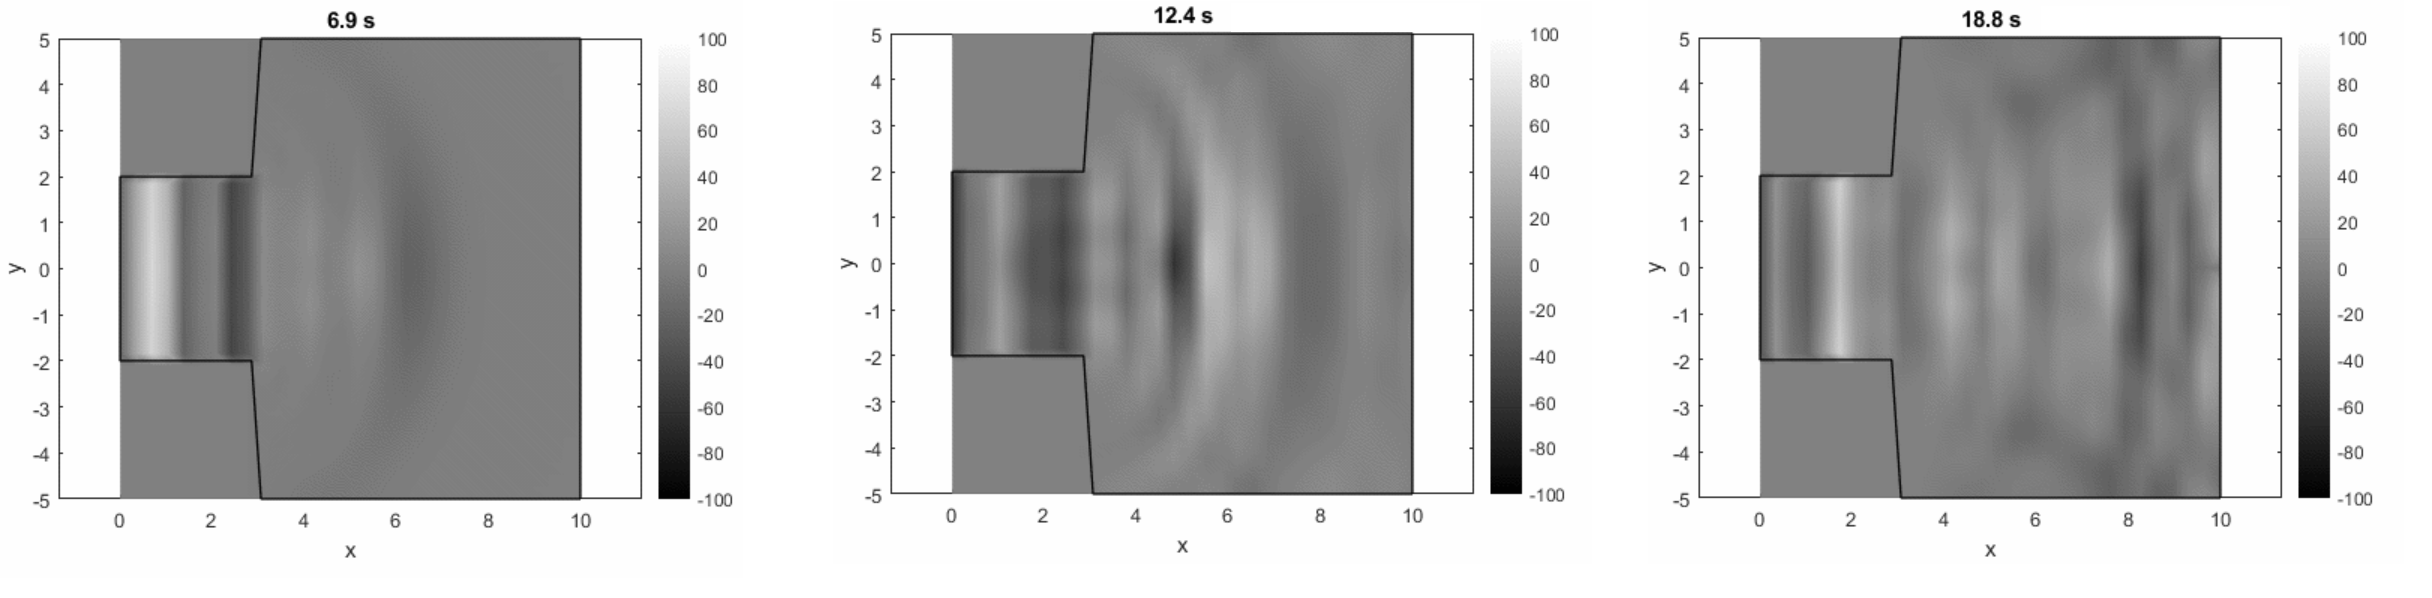
\includegraphics[width=\linewidth]{color_backstep.png}
\caption{Time evolution of the propagating wave in the `Backstep' geometry}
\label{fig:color backstep}
\end{figure}

\begin{figure}[ht]\centering % Using \begin{figure*} makes the figure take up the entire width of the page
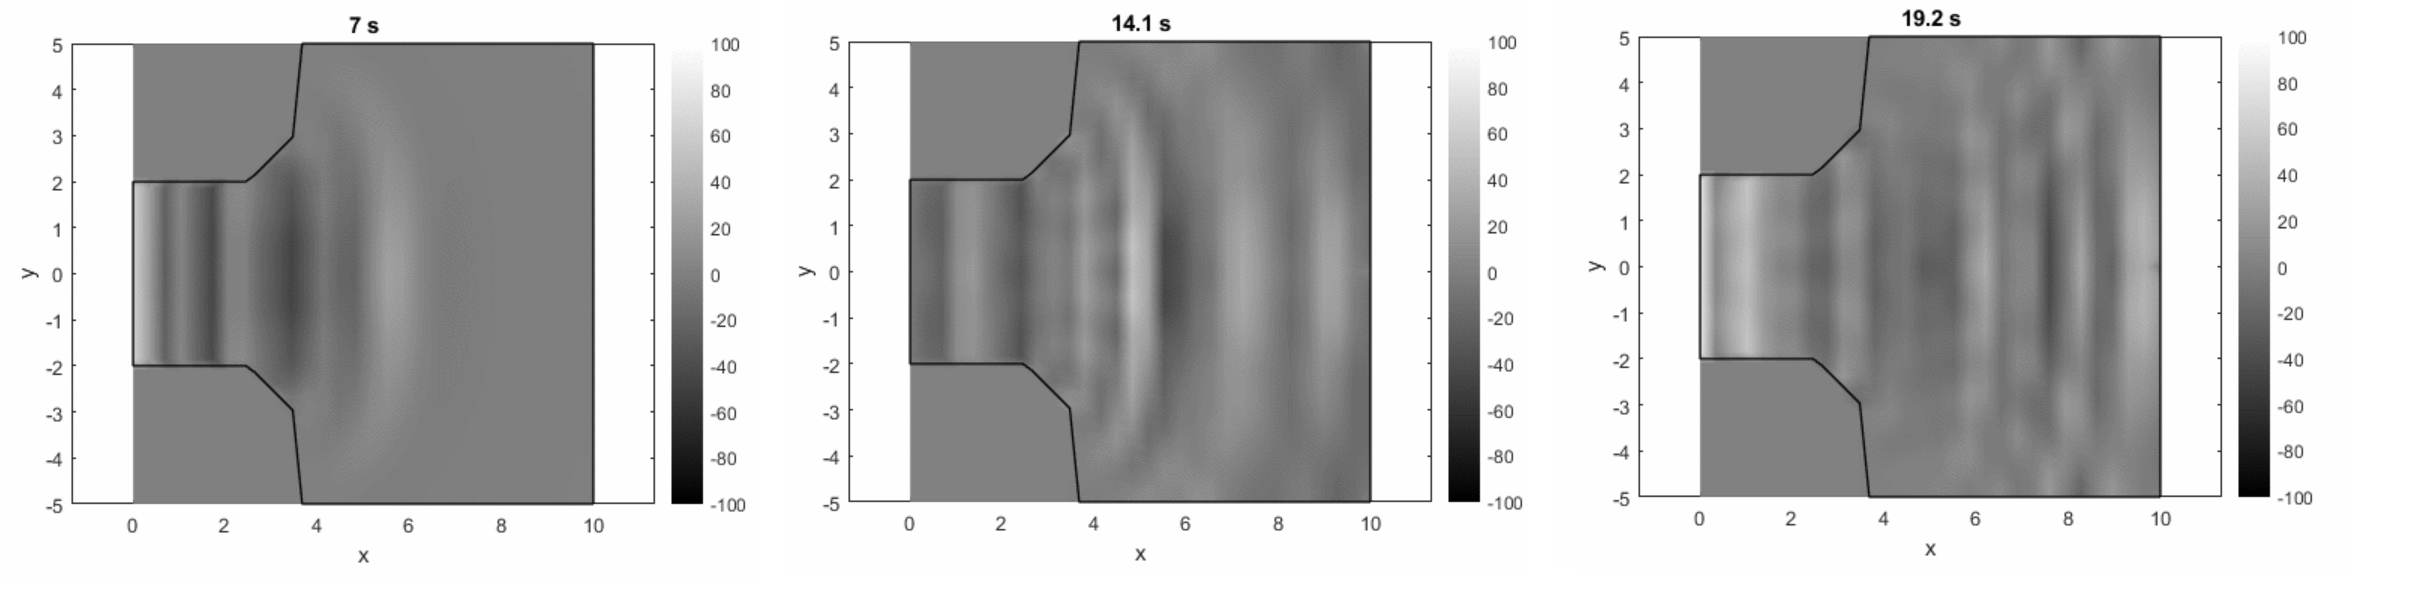
\includegraphics[width=\linewidth]{color_angledbackstep.png}
\caption{Time evolution of the propagating wave in the `angled Backstep' geometry}
\label{fig:color angledbackstep}
\end{figure}

\begin{figure}[ht]\centering % Using \begin{figure*} makes the figure take up the entire width of the page
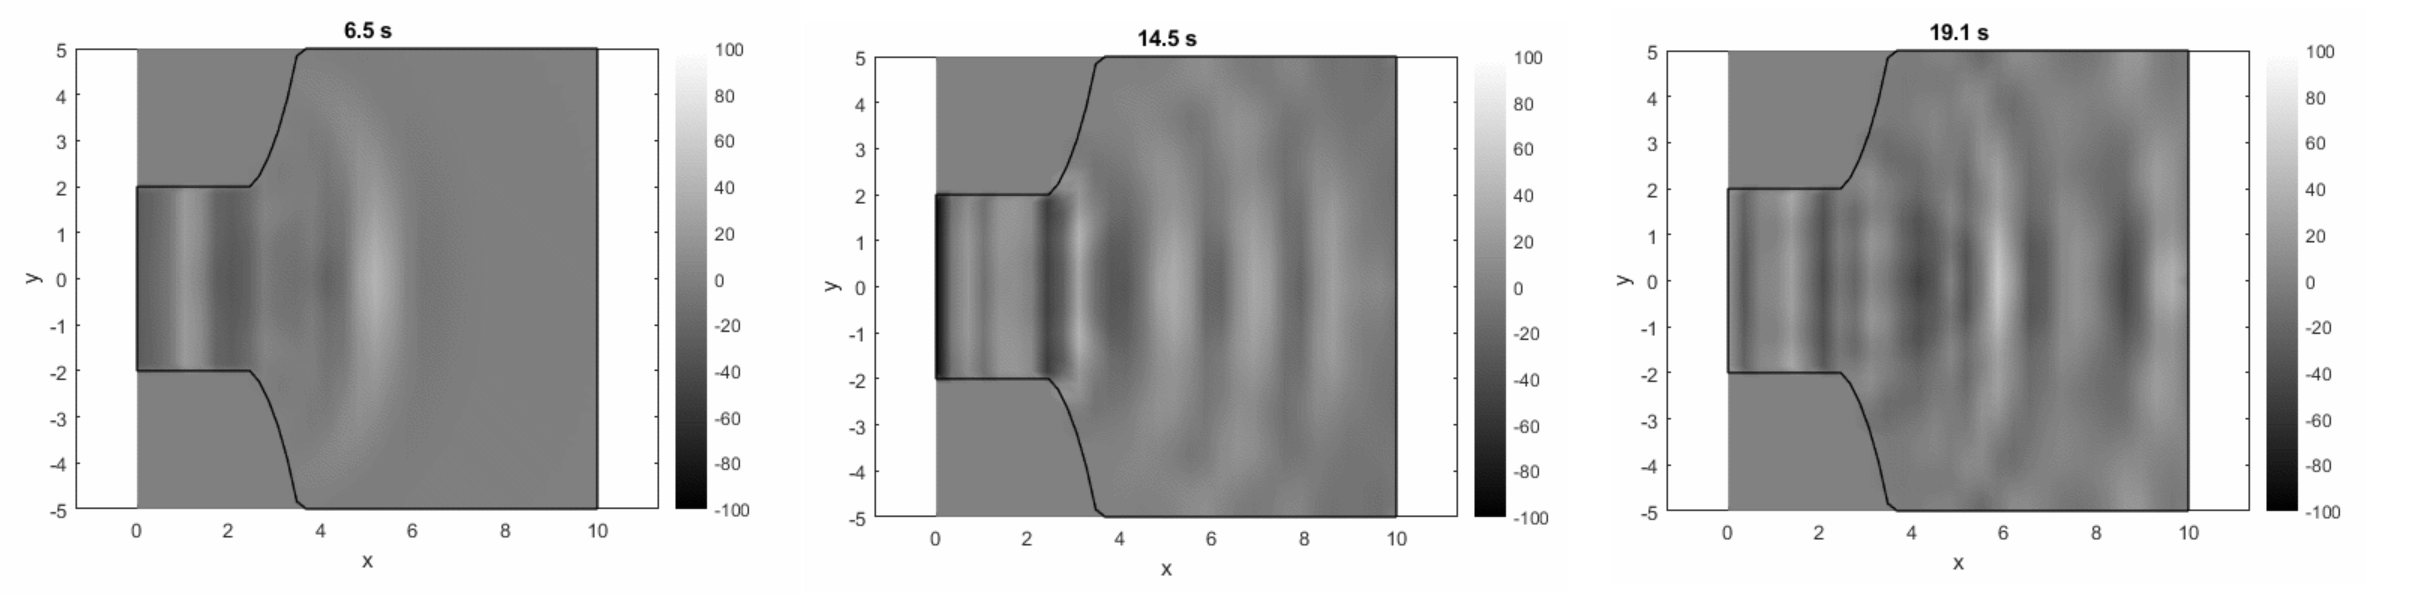
\includegraphics[width=\linewidth]{color_smoothoutlet.png}
\caption{Time evolution of the propagating wave in the `smooth Outlet' geometry}
\label{fig:color smoothoutlet}
\end{figure}

The time needed for the signal to reach the east (open) boundary as well as the the time needed for the signal to reach the higher volume outlet chamber is given in Tab.~ \ref{tab:time outlet} and \ref{tab:time inlet}.


\begin{table}[ht!]
\caption{Time needed to reach outlet}
\centering
\begin{tabular}{llr}
\toprule
\multicolumn{2}{c}{Parameter choice: $dt = 0.1$, $tend = 20$, $c = 1$} \\
\cmidrule(r){1-2}
Geometry & time in $[s]$ \\
\midrule
Backstep & $6.5 $ \\
angled Backstep & $6.5 $ \\
Smooth Outlet & $6.4 $ \\
\bottomrule
\end{tabular}
\label{tab:time outlet}
\end{table}

\begin{table}[ht!]
\caption{Time needed to leave inlet tube}
\centering
\begin{tabular}{llr}
\toprule
\multicolumn{2}{c}{Parameter choice: $dt = 0.1$, $tend = 20$, $c = 1$} \\
\cmidrule(r){1-2}
Geometry & time in $[s]$ \\
\midrule
Backstep & $1.0 $ \\
angled Backstep & $1.2 $ \\
Smooth Outlet & $1.2 $ \\
\bottomrule
\end{tabular}
\label{tab:time inlet}
\end{table}

\clearpage

\subsection{Probe Analysis}
Two probes where placed in the inlet tube and the outlet chamber to alow a quantitative analysis of the time evolution of the wave and its frequency spectrum. The probe positions are depicted in Fig.~\ref{fig:probe positions}. The instationary pressure probes are analysed for the time interval $t \in [0, 500]$. This rather long time intervall ensures that the wave can propagrate throughout the geometry and one takes account for the interference effects occuring due to the geometrical shape.

\begin{figure}[ht]\centering % Using \begin{figure*} makes the figure take up the entire width of the page
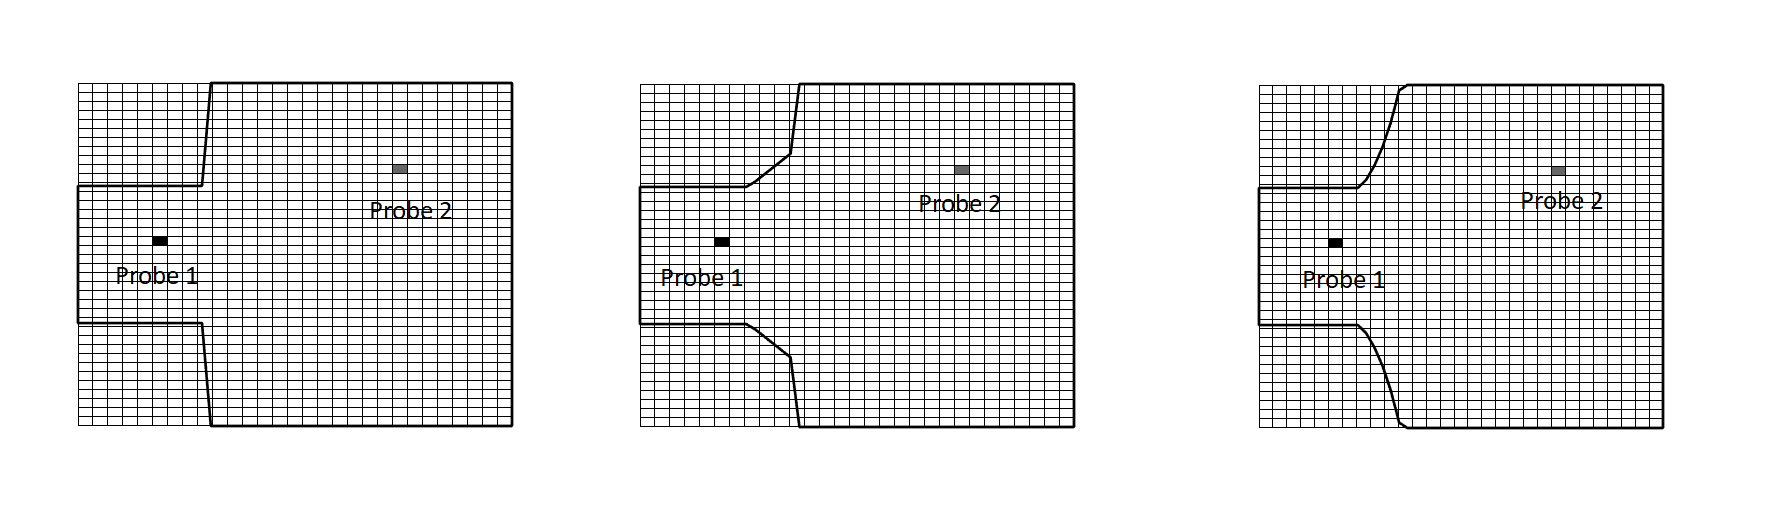
\includegraphics[width=\linewidth]{probe_positions.png}
\caption{Probe positions for time and spectral analysis}
\label{fig:probe positions}
\end{figure}

In Fig.~\ref{fig:spectral backstep inlet} one can see that a predominant frequency of approximately $0.1 \ Hz$ is monitored at the inlet probe. Due to the low angular frequency of the propagating wave the frequency range is depicted from $0-1 \ Hz$. The spectrum for the outlet probe in Fig.~\ref{fig:spectral backstep outlet} shows that other frequencies parts are developed in the outlet chamber. By comparison of both time signals in Fig.~\ref{fig:spectral backstep inlet} and \ref{fig:spectral backstep outlet} it is obvious that the amplitude is damped. This result is also reflected in the mean absolute amplitude values in Tab.~\ref{tab:meanvalues inlet} and \ref{tab:meanvalues outlet}. 

For the `angled Backstep' geometry multiple frequency components are found at the inlet probe. Likewise multiple frequency components are observed at the outlet chamber probe. However the spectra of inlet and outlet probe vary significantly. Therefore we conclude that for geometries `Backstep' and `angled Backstep' different frequencies are developed in the inlet tube as emitted through the outlet chamber. For the spectrum of the inlet probe of the `smooth Outlet' Geometry shows again the predominant frequency component is again found at approx. $0.1 \ Hz$. This frequency is also predominant in the spectrum at the outlet probe.

% time plot, spectrum backstep, inlet 
\begin{figure}[H]
\centering
\begin{subfigure}{.5\textwidth}
  \centering
  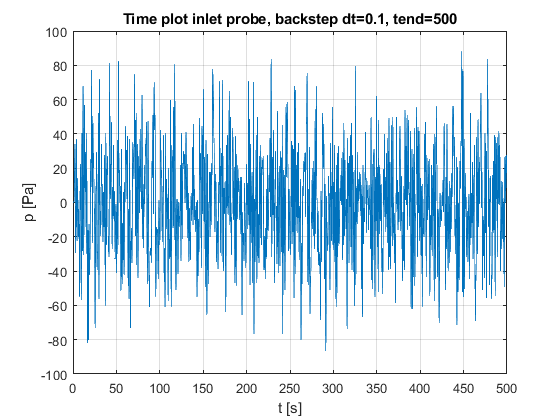
\includegraphics[width=.8\linewidth]{backstep_time_inlet.png}
  \caption{Plot of the amplitude over time}
  \label{fig:Plot of the amplitude over time}
\end{subfigure}%
\begin{subfigure}{.5\textwidth}
  \centering
  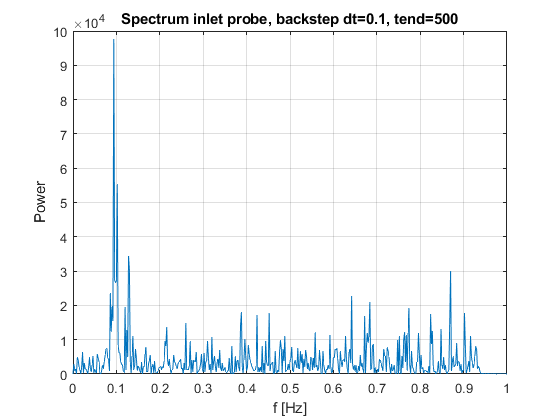
\includegraphics[width=.8\linewidth]{backstep_spectrum_inlet.png}
  \caption{Plot of the spectrum over the frequency}
  \label{fig:sub2}
\end{subfigure}
\caption{Spectral analysis of the inlet probe of the `Backstep' geometry}
\label{fig:spectral backstep inlet}
\end{figure}

% time plot, spectrum backstep, outlet
\begin{figure}[H]
\centering
\begin{subfigure}{.5\textwidth}
  \centering
  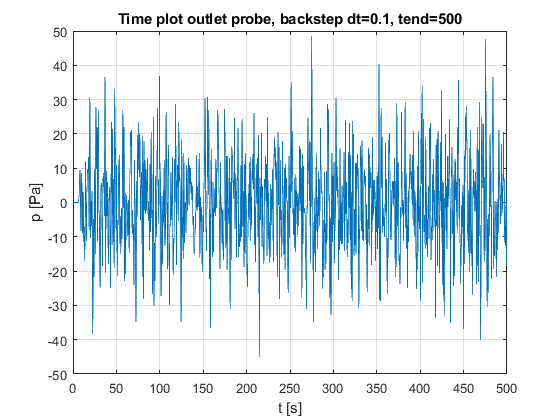
\includegraphics[width=.8\linewidth]{backstep_time_outlet.png}
  \caption{Plot of the amplitude over time}
  \label{fig:sub1}
\end{subfigure}%
\begin{subfigure}{.5\textwidth}
  \centering
  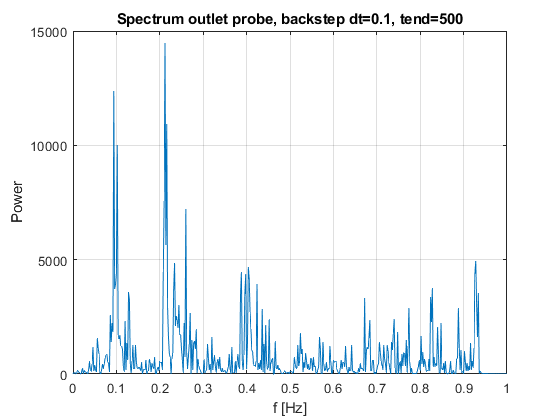
\includegraphics[width=.8\linewidth]{backstep_spectrum_outlet.png}
  \caption{Plot of the spectrum over the frequency}
  \label{fig:sub2}
\end{subfigure}
\caption{Spectral analysis of the outlet probe of the `Backstep' geometry}
\label{fig:spectral backstep outlet}
\end{figure}

% time plot, spectrum angled backstep, inlet
\begin{figure}[H]
\centering
\begin{subfigure}{.5\textwidth}
  \centering
  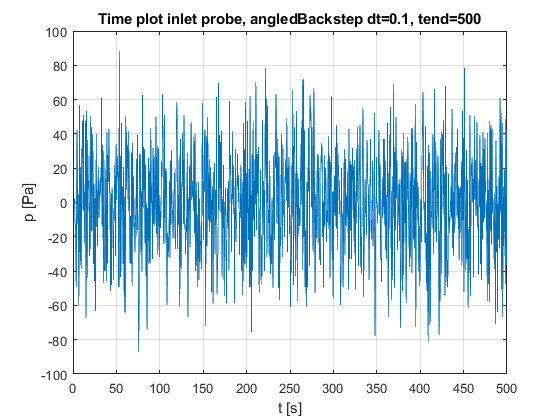
\includegraphics[width=.8\linewidth]{angledbackstep_time_inlet.png}
  \caption{Plot of the amplitude over time}
  \label{fig:sub1}
\end{subfigure}%
\begin{subfigure}{.5\textwidth}
  \centering
  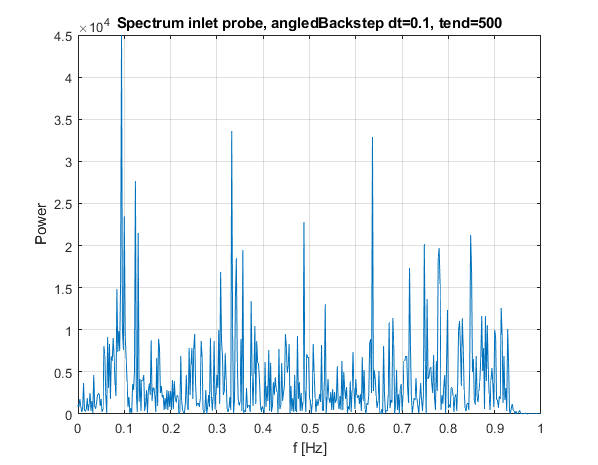
\includegraphics[width=.8\linewidth]{angledbackstep_spectrum_inlet.png}
  \caption{Plot of the spectrum over the frequency}
  \label{fig:sub2}
\end{subfigure}
\caption{Spectral analysis of the inlet probe of the `angled Backstep' geometry}
\label{fig:test}
\end{figure}

% time plot, spectrum angled backstep, outlet
\begin{figure}[H]
\centering
\begin{subfigure}{.5\textwidth}
  \centering
  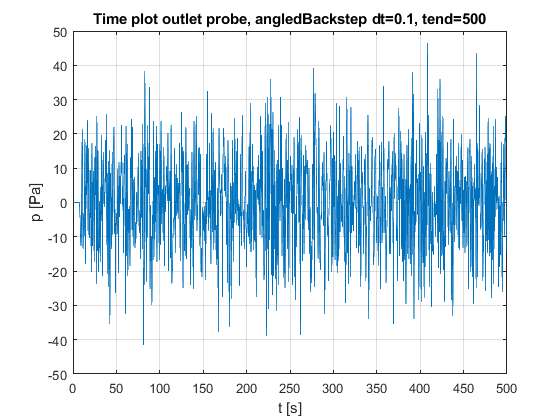
\includegraphics[width=.8\linewidth]{angledbackstep_time_outlet.png}
  \caption{Plot of the amplitude over time}
  \label{fig:sub1}
\end{subfigure}%
\begin{subfigure}{.5\textwidth}
  \centering
  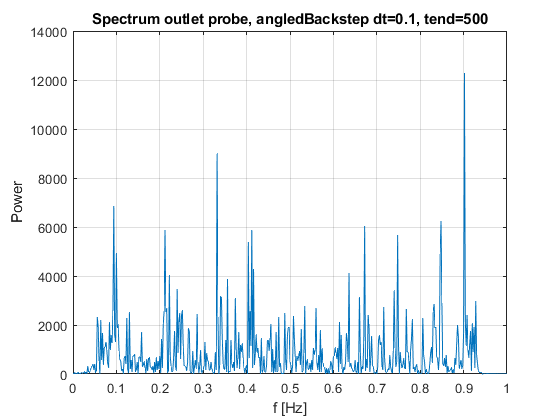
\includegraphics[width=.8\linewidth]{angledbackstep_spectrum_outlet.png}
  \caption{Plot of the spectrum over the frequency}
  \label{fig:sub2}
\end{subfigure}
\caption{Spectral analysis of the outlet probe of the `angled Backstep' geometry}
\label{fig:test}
\end{figure}

% time plot, spectrum smooth, inlet 
\begin{figure}[H]
\centering
\begin{subfigure}{.5\textwidth}
  \centering
  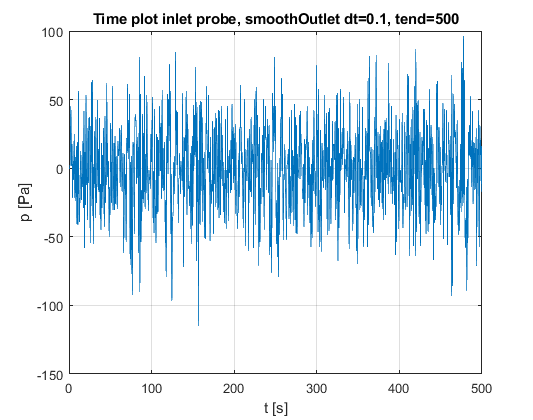
\includegraphics[width=.8\linewidth]{smooth_time_inlet.png}
  \caption{Plot of the amplitude over time}
  \label{fig:sub1}
\end{subfigure}%
\begin{subfigure}{.5\textwidth}
  \centering
  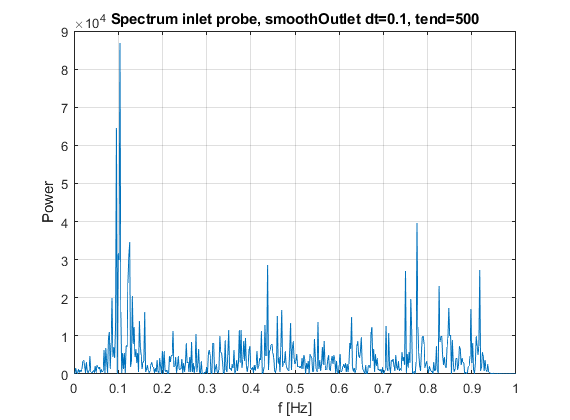
\includegraphics[width=.8\linewidth]{smooth_spectrum_inlet.png}
  \caption{Plot of the spectrum over the frequency}
  \label{fig:sub2}
\end{subfigure}
\caption{Spectral analysis of the inlet probe of the `smooth Outlet' geometry}
\label{fig:test}
\end{figure}

% time plot, spectrum smooth, outlet
\begin{figure}[H]
\centering
\begin{subfigure}{.5\textwidth}
  \centering
  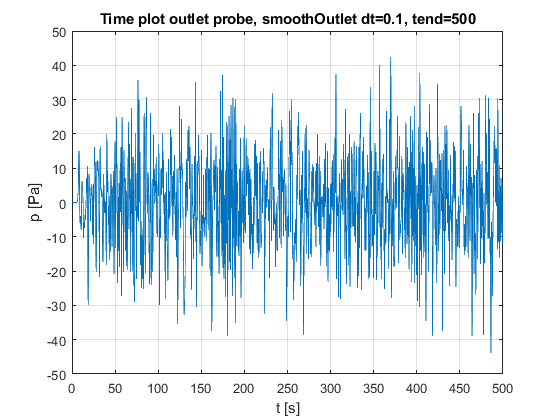
\includegraphics[width=.8\linewidth]{smooth_time_outlet.png}
  \caption{Plot of the amplitude over time}
  \label{fig:sub1}
\end{subfigure}%
\begin{subfigure}{.5\textwidth}
  \centering
  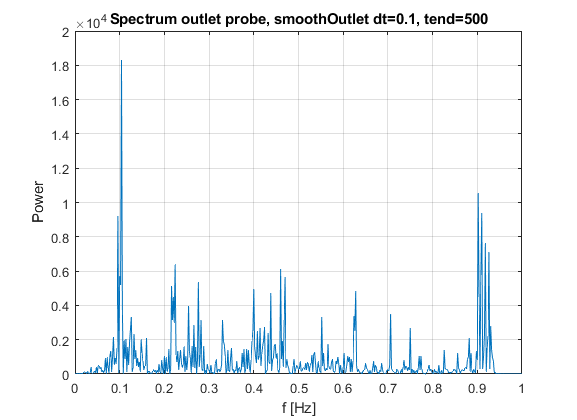
\includegraphics[width=.8\linewidth]{smooth_spectrum_outlet.png}
  \caption{Plot of the spectrum over the frequency}
  \label{fig:sub2}
\end{subfigure}
\caption{Spectral analysis of the outlet probe of the `smooth Outlet' geometry}
\label{fig:test}
\end{figure}


\begin{table}[ht!]
\caption{Maximum and mean absolute amplitudes for inlet probe}
\centering
\begin{tabular}{llr}
\toprule
\multicolumn{2}{c}{Inlet Probe} \\
\cmidrule(r){1-2}
Geometry & Mean value & Max value \\
\midrule 
Backstep  & 23.4877 & $102.0925$ \\
angled Backstep & 21.1267 & 84.8887 \\
Smooth Outlet  & 21.3841 & $96.4503$ \\
%Richard & Miles & $2$ \\
\bottomrule
\end{tabular}
\label{tab:meanvalues inlet}
\end{table}


\begin{table}[ht!]
\caption{Maximum and mean amplitudes for outlet probe}
\centering
\begin{tabular}{llr}
\toprule
\multicolumn{2}{c}{Probe Outlet} \\
\cmidrule(r){1-2}
Geometry & Mean value & Max value \\
\midrule

Backstep & 10.1596 & 45.1562 \\
angled Backstep & 9.8462 & 43.1932 \\
Smooth Outlet  & 9.4434 & $59.2770$ \\
\bottomrule
\end{tabular}
\label{tab:meanvalues outlet}
\end{table}



\section{Conclusions} % The \section*{} command stops section numbering
The overall solution of the 2d wave equation solver provides reasonable physical results, yet no concrete conclusions can be drawn regarding the physical reliability of the obtained results. As this study was performed without available experimental data, experimental evidence need to verify the observed behaviour in the studied geometries.

 Moreover, a more in-depth quantitative analysis is needed to monitor the solution of the solver. One could introduce multiple probes in the domain and also study excitations of fixed frequencies at the west boundary and their effect on the observed spectra. The possibility of a single frequency excitation is already provided in the code.  
 
 To cover more realistic physical behaviour the code could be extended for variable phase velocities $c(\vb{x})$. This would account for a wave travelling in different media or a medium of differing spatial physical properties. 



\section*{Acknowledgments} % The \section*{} command stops section numbering

\addcontentsline{toc}{section}{\hspace*{-\tocsep}Acknowledgments} % Adds this section to the table of contents with negative horizontal space equal to the indent for the numbered sections
We thank Dr. Camilo Silva for his support and valuable input throughout the project as well as for the insights in the theoretical and numerical aspects of computational fluid dynamics.


%----------------------------------------------------------------------------------------
%	REFERENCE LIST
%----------------------------------------------------------------------------------------

\bibliographystyle{unsrt}
\bibliography{bib}

%----------------------------------------------------------------------------------------

\end{document}